\section{验证：分子结构证据}

\begin{figure*}[t]
    \centering
    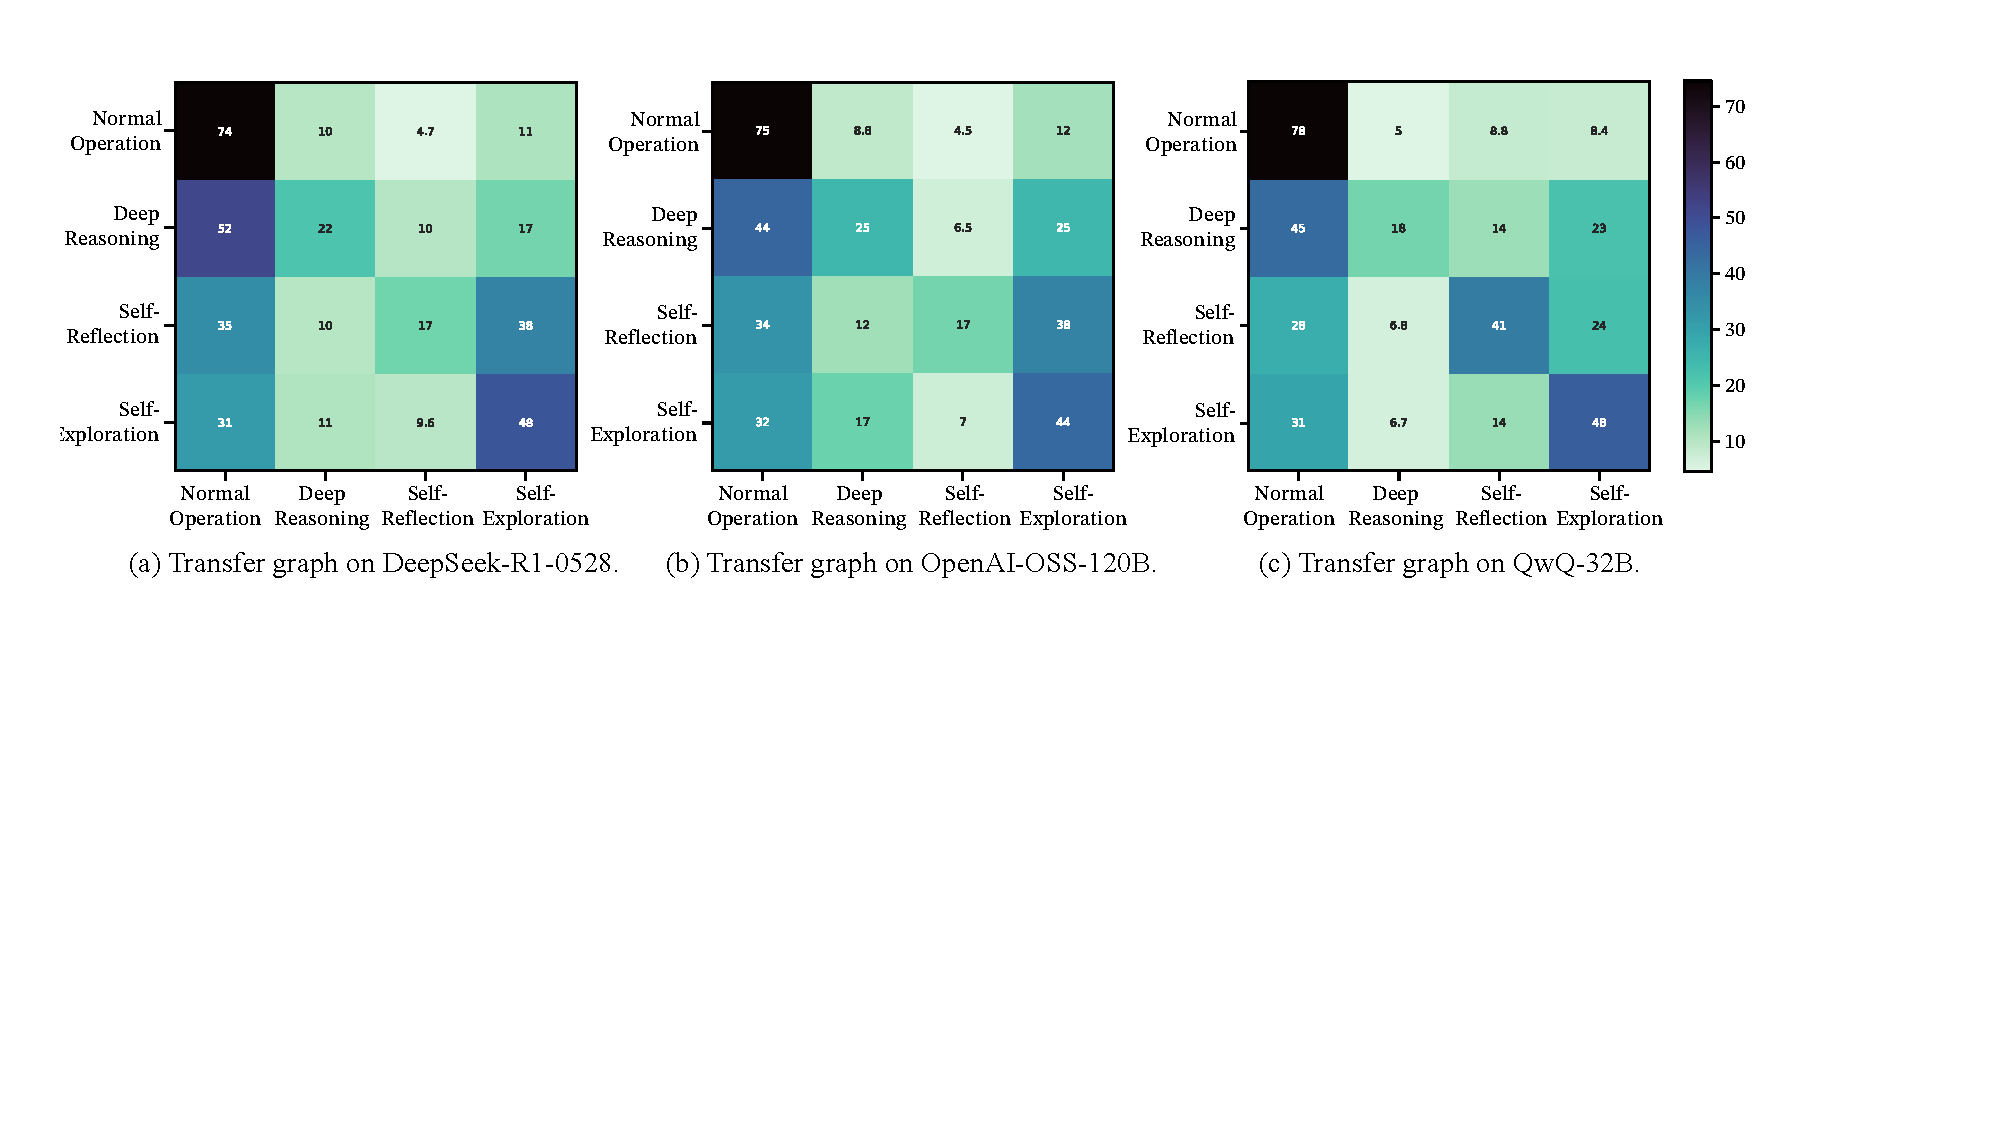
\includegraphics[width=0.98\textwidth]{figures/transfer.pdf}
    \caption{三个模型上的转移图。样本数超过 2,000 后，模型间皮尔逊相关系数均大于 0.9（p<0.001）；继续增加样本，转移图趋于稳定，不同采样规模间的相关系数可超过 0.95。}
    
    \label{fig:transfer}
\end{figure*}

\subsection{Long CoT 中的稳定键分布}
我们首先验证：有效的 Long CoT 轨迹在模型与任务上是否展现出类似大分子的稳定组织。图~\ref{fig:transfer} 表明，即便跨任务、跨模型采样，得到的轨迹在行为转移分布上的皮尔逊相关系数超过 0.9（p<0.001）。当样本多于 2,000 时，转移图在不同采样规模间的相关都超过 0.95。这说明，Long CoT 结构依赖于稳健的“基元”：不同模型都能在各类任务中恢复相似的推理拓扑，而简单的人类模拟或随机 ICL 无法复现这种全局键分布。

\subsection{SFT 学到的是这些键结构，而非关键词}
在 SFT 分析中，我们选用未在 Long CoT 数据上指令微调的 Llama-3.1-8B-Base；再对其用 R1 蒸馏数据训练，得到 Think-SFT 模型，即经过 Long CoT 强化的监督微调模型。\vspace{-8pt}




\begin{figure*}[t]
    \centering
    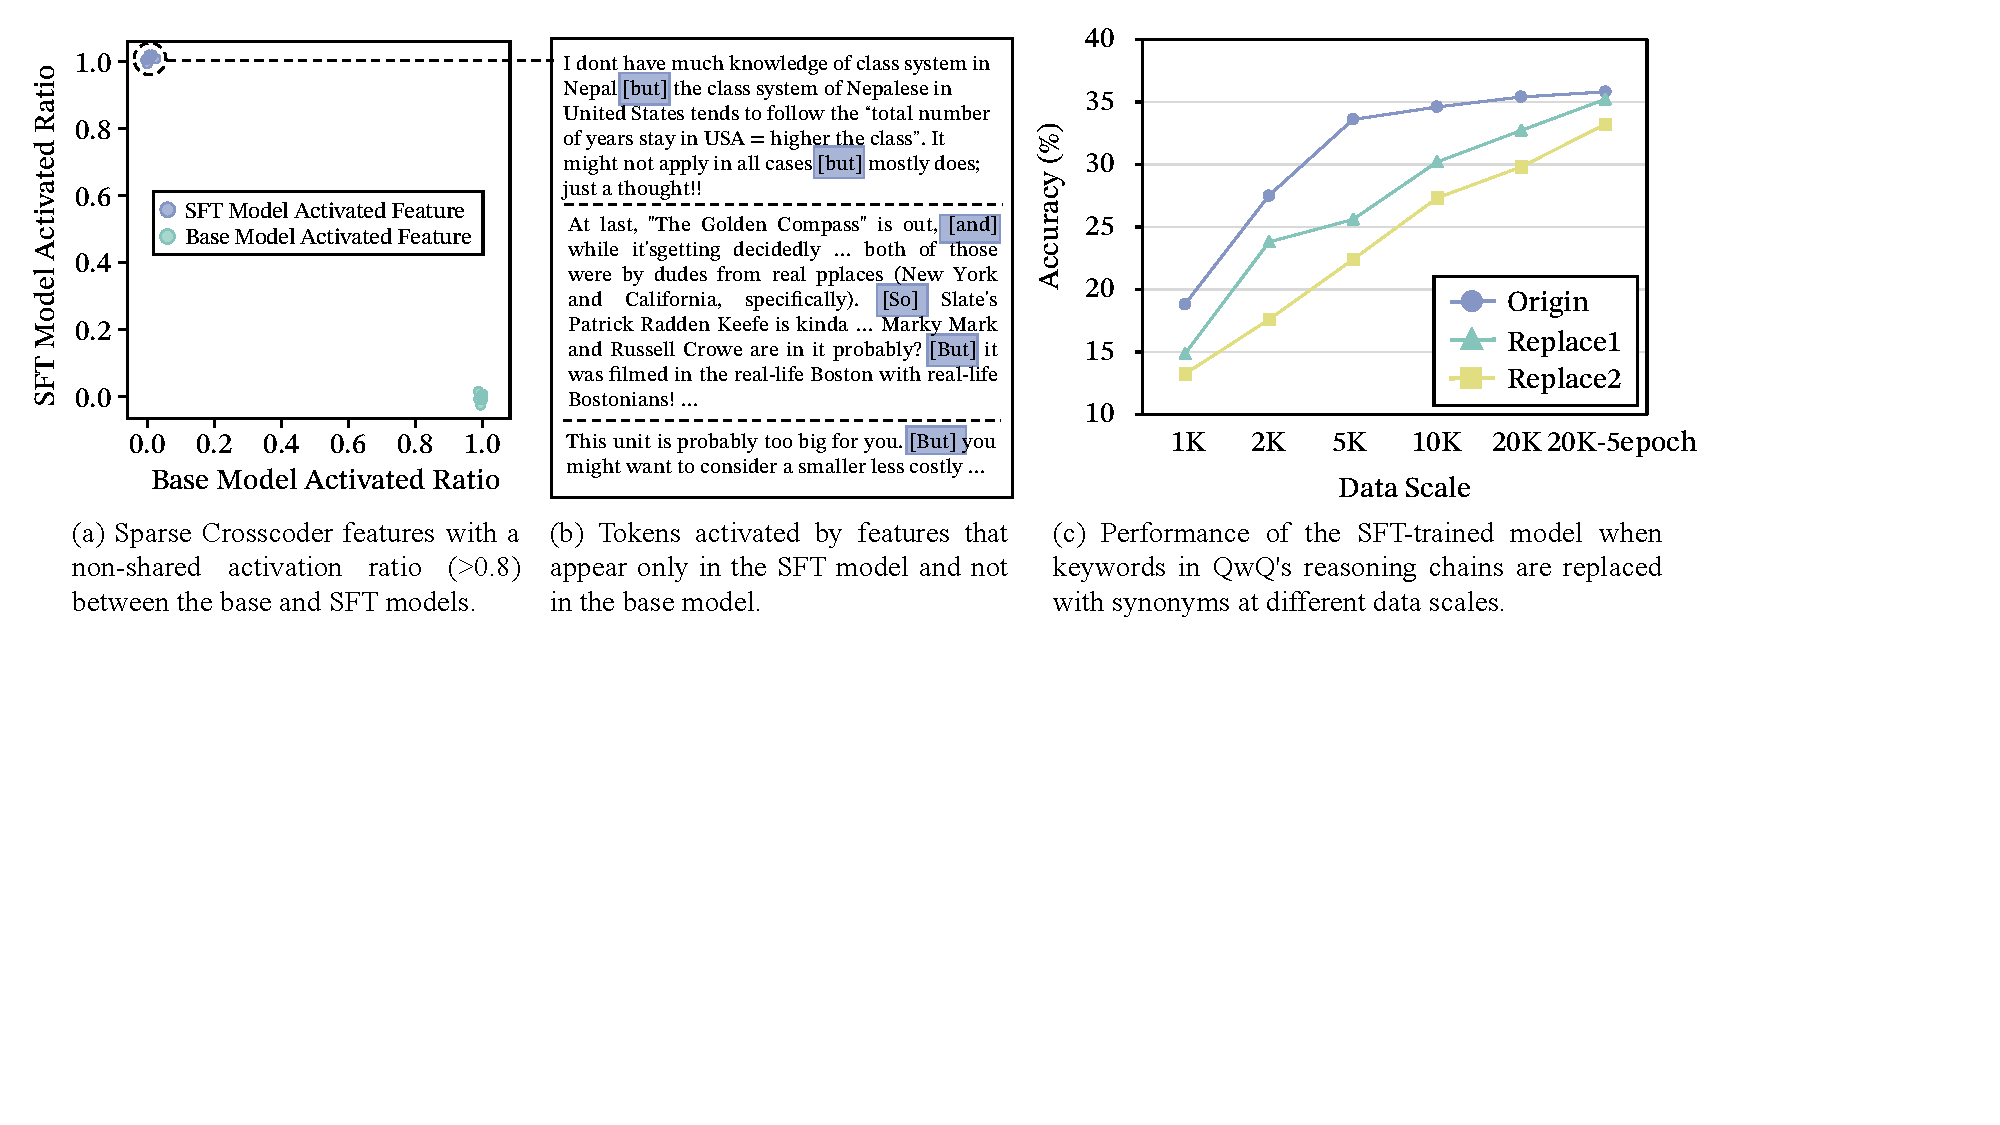
\includegraphics[width=0.98\textwidth]{figures/learning.pdf}
    \caption{Long CoT 监督微调中学到的特征。}
    \label{fig:learning}
\end{figure*}


从表征几何视角看，稀疏自编码器表明 Long CoT 行为集中在少量话语控制结构上，而非均匀分布于 token。图~\ref{fig:learning}(a,b) 所示，我们训练一个交叉编码稀疏自编码器，同时建模基座与 Think-SFT 模型的隐状态，再挑选那些在 think token 上激活率至少是平均水平三倍的特征。在这些高激活特征中，许多都由“Maybe”“But/so”“Alternatively”等逻辑连词触发，说明 SFT 刻意为长链推理中的局部假设修正、对比动作、分支选择等开辟了专门潜变量。

基于先前分析，我们认为模型学习的是这些关键词承载的推理行为，而非词面本身。遵循 \citet{chen2025towards} 给出的三类 Long CoT 推理行为，我们使用两份由 QwQ 蒸馏数据衍生的数据集来验证：第一份用四种替代说法替换每个关键词；第二份则直接移除所有关键词，仅保留推理轨迹。我们对两份数据训练相同的 LLM，并评估其 Long CoT 性能。

如图~\ref{fig:learning}(c) 所示，明确的关键词能加速学习，但不是必须的。只要保留底层推理行为，即便去掉关键词或随机替换，模型在充分训练后也能达到相当的推理表现。这一发现揭示：LLM 内化的是推理结构，而不是表面词汇。因此，若要真正增强推理能力，训练数据应优先匹配推理行为的分布，而非拘泥于特定关键词。

然而，一个关键问题仍待回答：这些“键”是否驱动 Long CoT 的结构学习？如果是，\textit{\textbf{为何显式模仿人类或随机 ICL 标记往往失败？}}







\begin{figure*}[t]
    \centering
    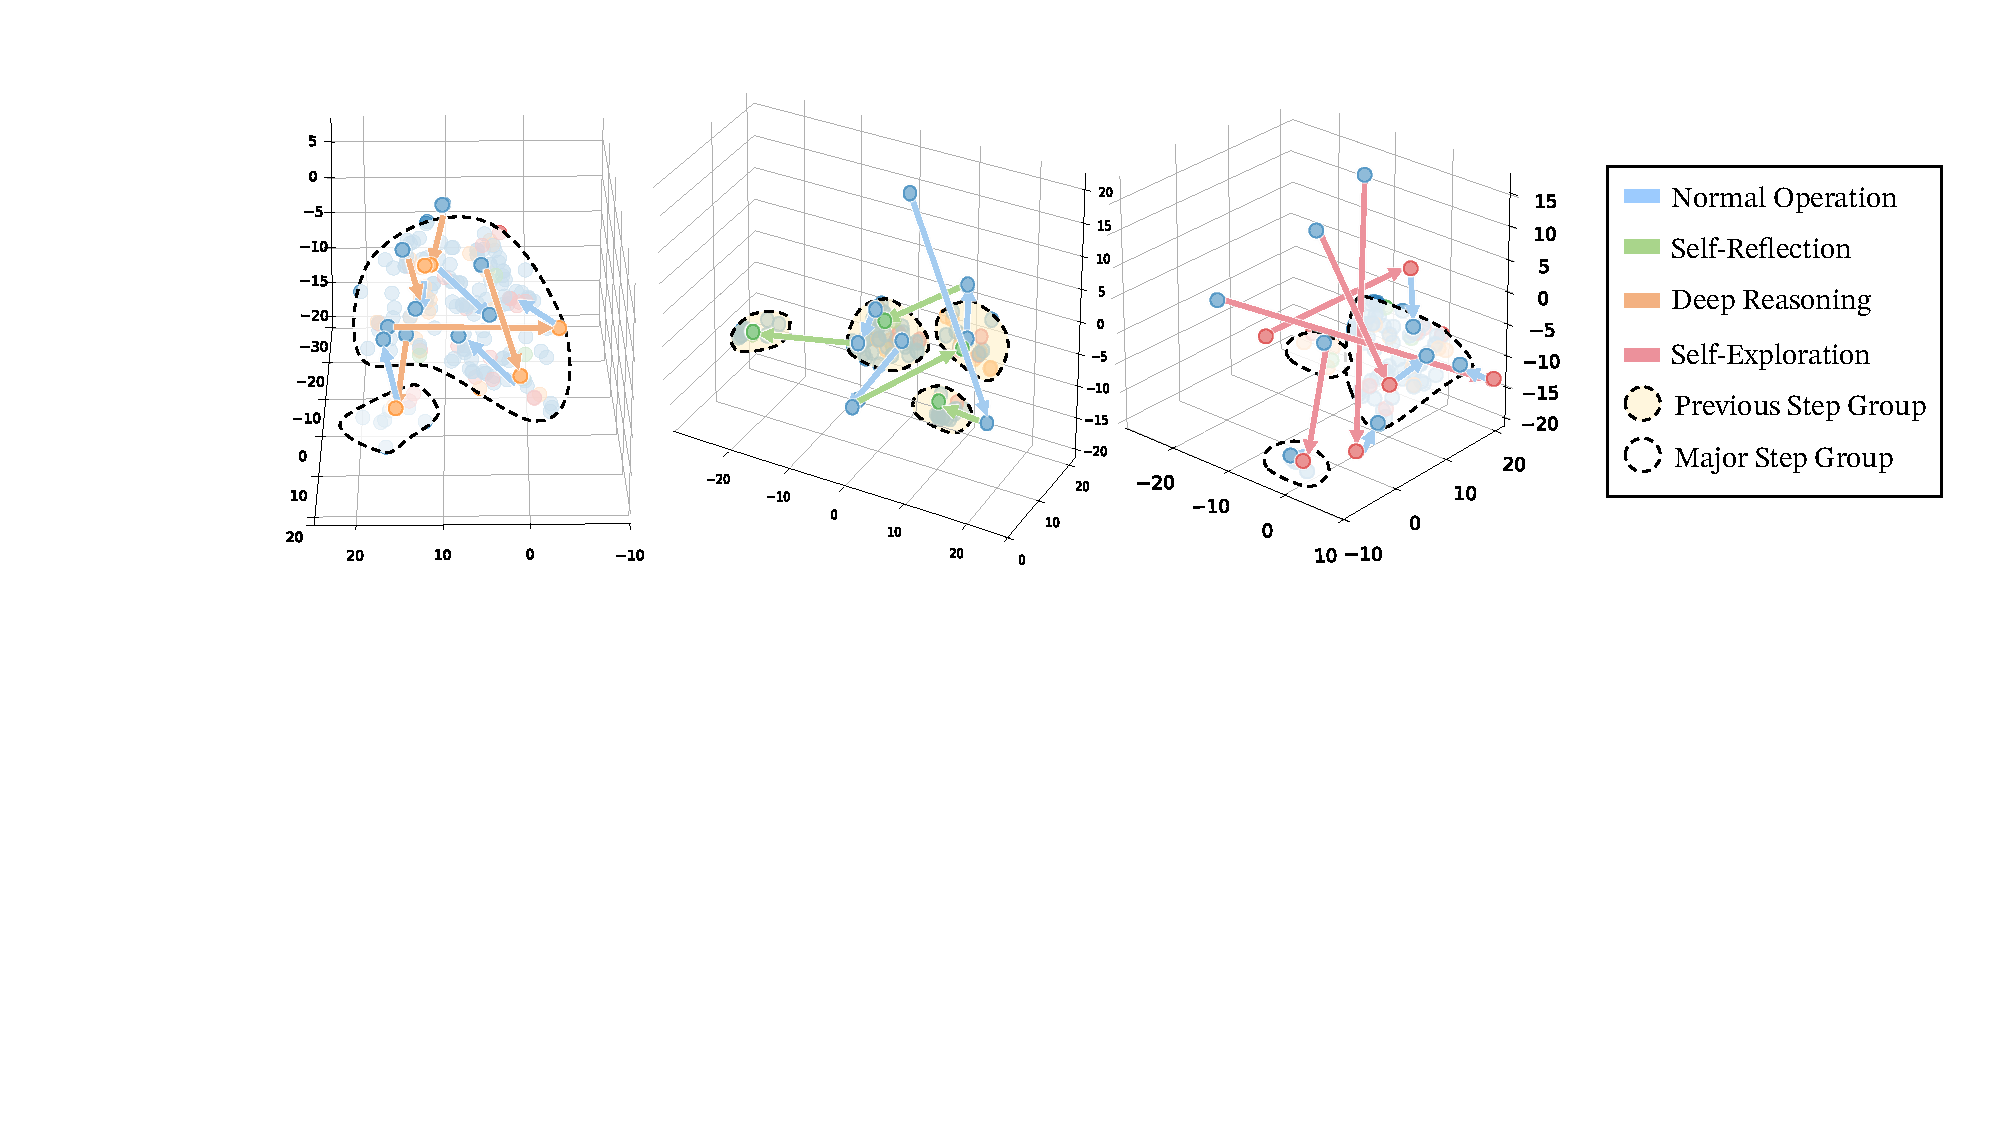
\includegraphics[width=0.96\textwidth]{figures/validation.pdf}
    \caption{在 Qwen2.5-32B-Instruct 的嵌入与 OpenAI-OSS-120B 推理过程的 t-SNE 低维表示上，验证“逻辑折叠”结构。}
    
    \label{fig:validation}
\end{figure*}

\begin{figure*}[t]
    \centering
    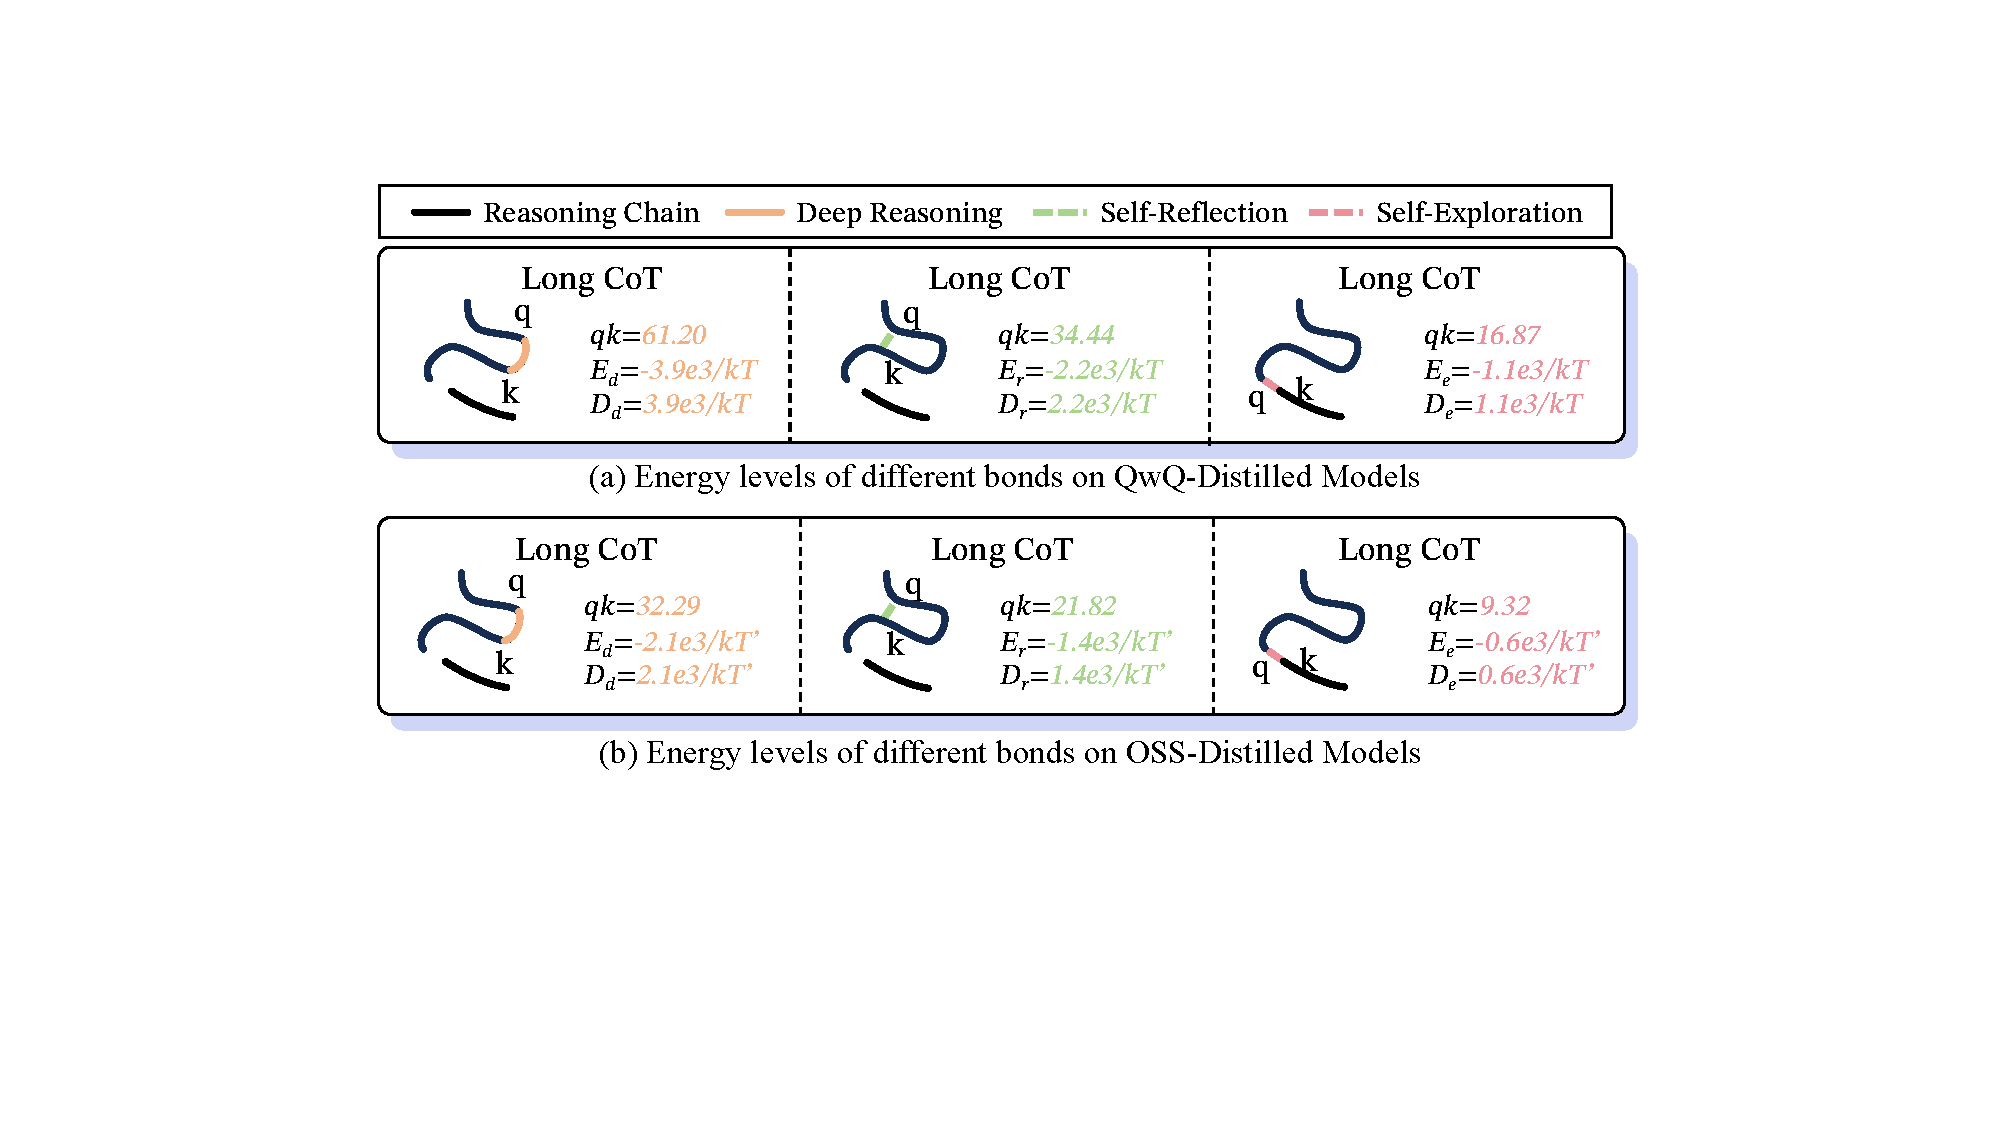
\includegraphics[width=0.76\textwidth]{figures/attention.pdf}
    
    \caption{两份蒸馏数据中不同键的能量水平。}
    
    \label{fig:attention}
\end{figure*}

\subsection{“逻辑键—折叠”结构}

为验证 Long CoT 类似宏观分子折叠的假设，我们在三维语义空间中分析了 CoT 的拓扑。我们把每条轨迹中的边标注为反思、深层推理或探索，并量化其几何属性。\vspace{-8pt}





\paragraph{\textbf{深层推理通过“共价键”稳固逻辑簇。}}
如图~\ref{fig:validation}(a)，深层推理键主要提升局部连通度，形成稳定子域。完成深层推理后，72.56\% 的步骤仍停留在语义空间距离小于 3 的同一簇内（而簇间距离通常大于 5.6）。\vspace{-8pt}

\paragraph{\textbf{自我反思以“氢键”形式折回先前步骤。}}
如图~\ref{fig:validation}(b)，自我反思把后续步骤折回早期且语义相似的簇，而非线性延伸链条。定量上，81.72\% 的反思步骤都会重连到先前形成的高相似簇。
\vspace{-8pt}

\paragraph{\textbf{自我探索以“范德华力”连接远距簇。}}
与局部稳固不同（图~\ref{fig:validation}(c)），自我探索在原本分离的簇之间创建松散链接。其步间距离显著更大，在 3D t-SNE 投影上的平均轨迹长度为 5.32。这些结果表明，有效 Long CoT 并非简单的线性链，而是形成了折叠、具有领域结构的拓扑，与“逻辑折叠”假设一致。




\subsection{注意力 $\Leftrightarrow$ 键的能级}
在物理化学中，温度 \(T\) 下能级为 $E_i$ 的状态概率满足玻尔兹曼分布：
\begin{equation}
    P(\text{state}_i) = \frac{\exp\!\big(-E_i / k_B T\big)}{\sum_j {\exp\!\big(-E_j / k_B T\big)}}.
    \label{eq:energy}
\end{equation}
Transformers 中，第 $i$ 个 token 对第 $j$ 个 token 的注意力权重 \(\alpha_{ij}\) 为：
\begin{equation}
\alpha_{ij} = \frac{\exp\!\big(q_i \cdot k_j / \sqrt{d_k}\big)}{\sum_l \exp\!\big(q_i \cdot k_l / \sqrt{d_k}\big)}.
\end{equation}
若定义注意力能量 $E = - q \cdot k$，则更低的 $E_{ij}$ 意味着更高的行为概率。

形式上，我们只需注意：注意力权重本质上是负 logits 的 Gibbs–Boltzmann 分布。因此，我们用“能量”表示重参数化后的 logits，并比较不同行为类型的期望值。


\begin{table*}[t]
\centering
\resizebox{0.96\textwidth}{!}{%
\begin{tabular}{lcccccccc}
\toprule
    \textbf{Model} & \textbf{GSM8K} & \textbf{MATH-500} & \textbf{AIME2024} & \textbf{AIME2025} & \textbf{AMC2023} & \textbf{OlympiadBench} & \textbf{AVG} \\
    \midrule
    LLaMA-3.1-8B-Base~\citep{dubey2024llama} & 7.58 & 3.20 & 0.00 & 0.00 & 4.22 & 1.19 & 2.70 \\
    \texttt{\ \ + 20K R1-Distill-Data} & 63.38 & 30.60 & 0.21 & 0.42 & 14.22 & 8.30 & 19.52 \\
    \texttt{\ \ + 20K OSS-Distill-Data} & 75.89 & 54.20 & 4.38 & 6.46 & 37.34 & 23.85 & 33.69 \\
    \texttt{\ \ + 20K QwQ-Distill-Data} & 64.53 & 32.20 & 2.92 & 0.42 & 16.72 & 8.89 & 20.95 \\
    \midrule
    Llama-3.1-8B-Instruct~\citep{dubey2024llama} & 75.89 & 35.20 & 4.17 & 1.04 & 23.59 & 12.00 & 25.32 \\
    \texttt{\ \ + 20K R1-Distill-Data}& 79.91 & 60.60 & 2.50 & 3.88 & 33.13 & 23.85 & 33.98 \\
    \texttt{\ \ + 20K OSS-Distill-Data} & 79.00 & 60.80 & 10.83 & 7.71 & 47.03 & 30.22 & 39.27 \\
    \texttt{\ \ + 20K QwQ-Distill-Data} & 82.41 & 60.80 & 4.38 & 8.33 & 32.97 & 25.48 & 35.73 \\
\bottomrule
\end{tabular}
}

\caption{六个基准的结果。完整结果见附录表~\ref{tab:full_distill_result}。}

\label{tab:distill_result}
\end{table*}
我们比较不同 Long CoT 转移类型的注意力能量。图~\ref{fig:attention} 显示，深层推理、反思与探索的能量分布截然不同：深层推理拥有最大的有效“化学键能量” $D_d$；反思居中，探索最弱。这种排序及其相对比例在不同模型中都一致，进一步支持了“键”机制广泛连接这些推理行为的假设。




\begin{TakeawayBox}{结论 2}
\begin{itemize}[leftmargin=16pt, itemsep=0pt, topsep=0pt]
    \item Long CoT 推理跨模型展现稳定结构，拓扑会收敛到相似形态；
    \item 语义异构体虽然访问相同概念，但成败取决于键结构，而非表面关键词；
    \item 三类逻辑键驱动 CoT 结构：反思折返过往簇，深层推理创建稳定局部域，探索桥接远距离概念；它们的注意力能量符合玻尔兹曼式分布；
    \item SFT 学到的是推理结构，而非词面，从根本上决定了 Long CoT 能力。
\end{itemize}
\end{TakeawayBox}
